%%
%% Automatically generated file from Doconce source
%% (http://code.google.com/p/doconce/)
%%
% #ifdef PTEX2TEX_EXPLANATION
%%
%% The file follows the ptex2tex extended LaTeX format, see
%% ptex2tex: http://code.google.com/p/ptex2tex/
%%
%% Run
%%      ptex2tex myfile
%% or
%%      doconce ptex2tex myfile
%%
%% to turn myfile.p.tex into an ordinary LaTeX file myfile.tex.
%% (The ptex2tex program: http://code.google.com/p/ptex2tex)
%% Many preprocess options can be added to ptex2tex or doconce ptex2tex
%%
%%      ptex2tex -DMINTED -DPALATINO -DA6PAPER -DLATEX_HEADING=traditional myfile
%%      doconce ptex2tex myfile -DMINTED -DLATEX_HEADING=titlepage
%%
%% ptex2tex will typeset code environments according to a global or local
%% .ptex2tex.cfg configure file. doconce ptex2tex will typeset code
%% according to options on the command line (just type doconce ptex2tex to
%% see examples).
% #endif

% #ifndef LATEX_HEADING
% #define LATEX_HEADING
% #endif

% #ifndef PREAMBLE
% #if LATEX_HEADING == "Springer_collection"
% #undef PREAMBLE
% #else
% #define PREAMBLE
% #endif
% #endif


% #ifdef PREAMBLE
%-------------------- begin preamble ----------------------

\documentclass[%
oneside,                 % oneside: electronic viewing, twoside: printing
final,                   % or draft (marks overfull hboxes)
10pt]{article}

\listfiles               % print all files needed to compile this document

% #ifdef A4PAPER
\usepackage[a4paper]{geometry}
% #endif
% #ifdef A6PAPER
% a6paper is suitable for mobile devices
\usepackage[%
  a6paper,
  text={90mm,130mm},
  inner={5mm},           % inner margin (two sided documents)
  top=5mm,
  headsep=4mm
  ]{geometry}
% #endif

\usepackage{relsize,epsfig,makeidx,color,amsmath,amsfonts}
\usepackage[latin1]{inputenc}
\usepackage{ptex2tex}

% #ifdef MINTED
\usepackage{minted}
\usemintedstyle{default}
% #endif

% #ifdef HELVETICA
% Set helvetica as the default font family:
\RequirePackage{helvet}
\renewcommand\familydefault{phv}
% #endif
% #ifdef PALATINO
% Set palatino as the default font family:
\usepackage[sc]{mathpazo}    % Palatino fonts
\linespread{1.05}            % Palatino needs extra line spread to look nice
% #endif

% Hyperlinks in PDF:
\usepackage[%
    colorlinks=true,
    linkcolor=black,
    %linkcolor=blue,
    citecolor=black,
    filecolor=black,
    %filecolor=blue,
    urlcolor=black,
    pdfmenubar=true,
    pdftoolbar=true,
    urlcolor=black,
    %urlcolor=blue,
    bookmarksdepth=3   % Uncomment (and tweak) for PDF bookmarks with more levels than the TOC
            ]{hyperref}
%\hyperbaseurl{}   % hyperlinks are relative to this root

\setcounter{tocdepth}{2}  % number chapter, section, subsection

% Tricks for having figures close to where they are defined:
% 1. define less restrictive rules for where to put figures
\setcounter{topnumber}{2}
\setcounter{bottomnumber}{2}
\setcounter{totalnumber}{4}
\renewcommand{\topfraction}{0.85}
\renewcommand{\bottomfraction}{0.85}
\renewcommand{\textfraction}{0.15}
\renewcommand{\floatpagefraction}{0.7}
% 2. ensure all figures are flushed before next section
\usepackage[section]{placeins}
% 3. enable begin{figure}[H] (often leads to ugly pagebreaks)
%\usepackage{float}\restylefloat{figure}

\newenvironment{exercise}{}{}
\newcounter{exerno}



% insert custom LaTeX commands...

\makeindex

%-------------------- end preamble ----------------------

\begin{document}

% #endif


% ------------------- main content ----------------------



% ----------------- title -------------------------
% #if LATEX_HEADING == "traditional"

\title{Using Web Frameworks for Scientific Web Applications}

% #elif LATEX_HEADING == "titlepage"

\thispagestyle{empty}
\hbox{\ \ }
\vfill
\begin{center}
{\huge{\bfseries{Using Web Frameworks for Scientific Web Applications}}}

% #elif LATEX_HEADING == "Springer_collection"

\title*{Using Web Frameworks for Scientific Web Applications}
% Short version of title:
%\titlerunning{...}

% #else

\begin{center}
{\LARGE\bf Using Web Frameworks for Scientific \\ [1.5mm] Web Applications}
\end{center}

% #endif

% ----------------- author(s) -------------------------
% #if LATEX_HEADING == "traditional"
\author{Hans Petter Langtangen\footnote{Center for Biomedical Computing, Simula Research Laboratory and Department of Informatics, University of Oslo.}
\and Anders Johansen\footnote{Center for Biomedical Computing, Simula Research Laboratory.}}

% #elif LATEX_HEADING == "titlepage"
\vspace{1.3cm}

    {\Large\textsf{Hans Petter Langtangen${}^{1, 2}$}}\\ [3mm]
    
    {\Large\textsf{Anders Johansen${}^{1}$}}\\ [3mm]
    
\ \\ [2mm]

{\large\textsf{${}^1$Center for Biomedical Computing, Simula Research Laboratory} \\ [1.5mm]}
{\large\textsf{${}^2$Department of Informatics, University of Oslo} \\ [1.5mm]}
% #elif LATEX_HEADING == "Springer_collection"

\author{Hans Petter Langtangen and Anders Johansen}
% Short version of authors:
%\authorrunning{...}
\institute{Hans Petter Langtangen\at Center for Biomedical Computing, Simula Research Laboratory and Department of Informatics, University of Oslo \and Anders Johansen\at Center for Biomedical Computing, Simula Research Laboratory}

% #else

\begin{center}
{\bf Hans Petter Langtangen${}^{1, 2}$} \\ [0mm]
\end{center}


\begin{center}
{\bf Anders Johansen${}^{1}$} \\ [0mm]
\end{center}

\begin{center}
% List of all institutions:
\centerline{{\small ${}^1$Center for Biomedical Computing, Simula Research Laboratory}}
\centerline{{\small ${}^2$Department of Informatics, University of Oslo}}
\end{center}
% #endif
% ----------------- end author(s) -------------------------


% ----------------- date -------------------------

% #if LATEX_HEADING == "traditional"

\date{Mar 22, 2013}
\maketitle

% #elif LATEX_HEADING == "titlepage"

\ \\ [10mm]
{\large\textsf{Mar 22, 2013}}

\end{center}
\vfill
\clearpage

% #else

\begin{center}
Mar 22, 2013
\end{center}

\vspace{1cm}

% #endif


\tableofcontents

\vspace{1cm} % after toc






\section{Web frameworks}

\index{web frameworks}

Computational scientists may want to offer their applications through
a web interface, thereby making a \emph{web application}.
Basically, this means that users can set input data
to the application on a web page, then click on some \emph{Compute} button,
and back comes a new web page with the results of the computations.
The web interface can either be used as a GUI locally on the
scientist's computer, or the interface can be depolyed to
a server and made available to the whole world.

Web applications of the mentioned type can be created from scratch
using CGI scripts in (e.g.) Python, but the code quickly gets longer
and more involved as the complexity of the web interface
grows. Nowadays, most web applications are created with the aid of
\emph{web frameworks}, which are software packages that simplify the
programming tasks of offering services through the Internet. The
downside of web frameworks is that there is a significant amount of
steps and details to learn before your first simple demo application
works.  The upside is that advanced applications are within reach,
without an overwhelming amount of programming, as soon as you have
understood the basic demos.

We shall explore two web frameworks: the very popular \href{{https://www.djangoproject.com/}}{Django framework} and the more high-level and easy-to-use framework
\href{{http://flask.pocoo.org/}}{Flask}. In addition, our examples are also
implemented in the \href{{http://www.web2py.com/}}{web2py} framework.
% Its slogan says "Django makes it easier to build better Web apps more quickly and with less code".
The primary advantage of Django
over other web frameworks is the rich set of documentation and
examples. Googling for "Django tutorials" gives lots of hits including
a  list of \href{{https://code.djangoproject.com/wiki/Tutorials}}{web tutorials}
and a list of \href{{http://www.youtube.com/playlist?list=PL385A53B00B8B158E}}{YouTube videos}. There is also an electronic \href{{http://www.djangobook.com/en/2.0/}}{Django book}. At the time of this writing, Flask is not
much documented beyond the \href{{http://flask.pocoo.org/}}{official web site} and the \href{{http://wtforms.simplecodes.com/docs/0.6/index.html}}{WTForms Documentation}. There is, unfortunately, hardly any examples on how Django or Flask can be used to enable typical scientific applications for the web, and that is why we have developed some targeted examples on this topic.


The problem for a computational scientist who wants to enable
mathematical calculations through the web is that most of
the introductory examples on utilizing a particular
web framework address web applications
of very different nature, e.g., blogs and polls. Therefore, we have made an
alternative introduction which explains, in the simplest possible way,
how web frameworks can be used to

\begin{enumerate}
\item generate a web page with input data to your application,

\item run the application to perform mathematical computations, and

\item generate a web page with the results of the computations.
\end{enumerate}

\noindent
To work with Django, you need to know about Python packages and modules
as well as Python classes. With Flask it is enough to be familiar with
functions and modules, though knowledge of classes and a bit of
decorators might be an advantage.

% !split
\subsection{The MVC pattern}

\index{MVC pattern}

The MVC pattern stands for Model-View-Controller and is a way of
separating the user's interaction with an application from the inner
workings of the application. In a scientific application this
usually means separaring mathematical computations from the
user interface and visualization of results.
The \href{{http://en.wikipedia.org/wiki/MVC_Pattern}}{Wikipedia definition of the MVC pattern} gives a very high-level
explanation of what the model, view, and controller do and mentions
the fact that different web frameworks interpret the three components
differently. Any web application works with a set of data and needs
a user interface for the communication of data between the user and
some data processing software. The classical
MVC pattern introduces

\begin{itemize}
 \item the model to hold the data

 \item the view to display data

 \item the controller to move data by gluing the model and the view.
\end{itemize}

\noindent
For applications performing mathematical computations we find it
convenient to explicitly introduce a fourth component that we call
\emph{compute} where the mathematical computations are encapsulated.  With
the MVC pattern and the compute component we have a clear separation
between data (model), the way data is presented (view), the
computations (compute), and the way these components communicate
(controller). In a small program such a separation may look as
overkill, but it pays off in more complicated applications. More
importantly, the concepts of the MVC pattern saturates the modules and
files of web frameworks so one really needs to adapt to the MVC way of
thinking.

Web frameworks often have their own way of interpreting the
model, view, and controller parts of the MVC pattern.
In particular, most frameworks often divide the view into two parts:
one software component and one HTML template. The latter takes care
of the look and feel of the web page while the former often takes
the role of being the controller too.
For our scientific applications
we shall employ an interpretation of the MVC pattern
which is compatible with what we need later on:

\begin{itemize}
 \item the model contains the data (often only the input data) of the application,

 \item the view controls the user interface that handles input and output data,
   and also calls to functionality that computes the output given the input.
\end{itemize}

\noindent
The model will be a Python class with static attributes holding the data.
The view consists of Python code processing the model's data and HTML
templates for the design of the web pages.

Flask does not force any MVC pattern on the programmer, but
the code needed to build web applications can easily be split into
model, view, controller, and compute components, as will be shown later.
Django, on the other hand, automatically generates application files with names
\code{views.py} and \code{models.py} so it is
necessary to have some idea what Django means with these terms.
The controller functionality in Django lies both in the \code{views.py} file and
in the configuration
files (\code{settings.py} and \code{urls.py}). The view component of the application
consists both of the \code{views.py} file and template files used to create
the HTML code in the web pages.

Forthcoming examples will illustrate how a scientific application is
split to meet the requirements of the MVC software design pattern.

% !split
\subsection{A very simple application}



We shall start with the simplest possible application,
a "scientific hello world program", where the
task is to read a number of write out "Hello, World!" followed by
the sine of the number. This application has one input variable and
a line of text as output.

Our first implementation reads the input from the command
line and writes the results to the terminal window:

\bpypro
#!/usr/bin/env python
import sys, math
r = float(sys.argv[1])
s = math.sin(r)
print "Hello, World! sin(%g)=%g' % (r, s)
\epypro

The task of the web version of this program is to read \code{r}
variable from a web page, compute the sine,
and write out a new web page with the resulting text.

% !split
\subsection{Application of the MVC pattern}
\label{wf:hw:mvc}



Before thinking of a web application, we first \emph{refactor} our program
such that it fits with the classical MVC pattern and a compute component.
The refactoring does not change the functionality of the code, it
just distributes the original statements in functions and modules.
Here we create four modules: \code{model}, \code{view},
\code{compute}, and \code{controller}.

\begin{itemize}
 \item The \code{compute} module contains a function \code{compute(r)} that performs
   the mathematics and returns the value of \code{s}.

 \item The \code{model} module holds the input data, here \code{r}.

 \item The \code{view} module has two functions, one for reading input data,
   \code{get_input},
   and one for presenting the output, \code{present_output}.
   The later takes the input, calls \code{compute} functionalty, and
   generates the output.

 \item The \code{controller} module initializes model's data from the view
   and calls the view to present the output.
\end{itemize}

\noindent
The \code{model.py} file contains the \code{r} variable, which must
be declared with a default value in order to create the data object:

\bpypro
r = 0.0    # input
s = None   # output
\epypro

The \code{view.py} file is restricted to the communication with the user and reads

\bpypro
import sys
import compute

# Input: float r
# Output: "Hello, World! sin(r)=..."

def get_input():
    """Get input data from the command line."""
    r = float(sys.argv[1])
    return r

def present_output(r):
    """Write results to terminal window."""
    s = compute.compute(r)
    print 'Hello, World! sin(%g)=%g' % (r, s)
\epypro

The mathematics is encapsulated in \code{compute.py}:

\bpypro
import math

def compute(r):
    return math.sin(r)
\epypro

Finally, \code{controller.py} glues the model and the view:

\bpypro
import model, view

model.r = view.get_input()
view.present_output(model.r)
\epypro

Let us try our refactored code:

\bsys
Terminal> python controller.py 1.2
Hello, World! sin(1.2)=0.932039
\esys

Our goal is to create a web interface to our scientific hello world
program such that we can fill in the number \code{r} in a text field, click a
\emph{Compute} button and get back a new web page with the output text
shown above: "Hello, World! sin(r)=s".

% !split
\section{Making a Flask application}

\index{Flask!installation}

Not much code or configuration is needed to make a Flask application.
Actually one short file is enough. For this file to work you need to
install Flask and some corresponding packages. This is easiest
performed by

\bsys
Terminal> sudo pip install Flask
Terminal> sudo pip install WTForms
\esys
You can add \code{--upgrade} to upgrade a previous installation.

\subsection{Programming the Flask application}

We want our input page to feature in text field where the user can
write the value of \code{r}, see Figure~\ref{wf:hw1:flask:fig:input}.
By clicking \emph{equals}
we compute the corresponding \code{s} and write out the result page
seen in Figure~\ref{wf:hw1:flask:fig:result}.


\begin{figure}[ht]
  \centerline{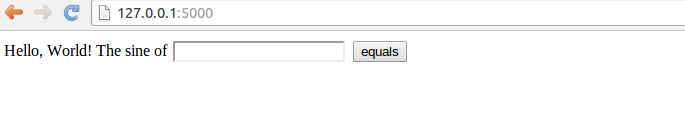
\includegraphics[width=0.9\linewidth]{fig-web4sa/hw1_flask_input.png}}
  \caption{
  The input page. \label{wf:hw1:flask:fig:input}
  }
\end{figure}
%\clearpage % flush figures wf:hw1:flask:fig:input



\begin{figure}[ht]
  \centerline{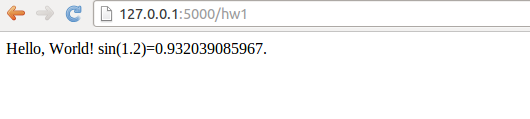
\includegraphics[width=0.9\linewidth]{fig-web4sa/hw1_flask_output.png}}
  \caption{
  The output page. \label{wf:hw1:flask:fig:result}
  }
\end{figure}
%\clearpage % flush figures wf:hw1:flask:fig:result




Flask does not require us to use the MVC pattern so there is actually
no need to split the original program into \code{model.py}, \code{view.py},
\code{controller.py}, and \code{compute.py} as already explained.  First we make
a \code{controller.py} file where the view, the model, and the controller
parts are within the same part. Later, we split the view, model, and
controller into three files for illustration. The \code{compute} component
is always in a separate files as we like to encapsulate the
computations completely from user interfaces.

\index{Flask!input forms}

The view that the user sees is determined by
HTML templates in a subdirectory \code{templates}, and consequently
we name the template files \code{view*.html}.
The model and other parts of the view concept are just parts of
the \code{controller.py} file:

\bpypro
from flask import Flask, render_template, request
from wtforms import Form, FloatField, validators
from compute import compute

app = Flask(__name__)

# Model
class InputForm(Form):
    r = FloatField(validators=[validators.InputRequired()])

# View
@app.route('/hw1', methods=['GET', 'POST'])
def index():
    form = InputForm(request.form)
    if request.method == 'POST' and form.validate():
        r = form.r.data
        s = compute(r)
        return render_template("view_output.html", form=form, s=s)
    else:
        return render_template("view_input.html", form=form)

if __name__ == '__main__':
    app.run(debug=True)
\epypro
We collect the files associated with a Flask app in a directory,
here called \code{hw1_flask}.

The web application is the \code{app} object of class \code{Flask} initialized
as shown. The model is a special Flask class derived from \code{Form}
where the data are listed as static class attributes and initialized
by various form field objects from the \code{wtforms} package.
These form fields correspond to HTML forms in the input page.
For the \code{r} variable we apply \code{FloatField} since it is a floating-point
variable. A default validator, here checking that the user supplies
a real number, is easily included.

The view, controlling how the user interacts with the data, consists
an URL and corresponding function to call when this is invoked URL.
The function name is here \code{index} (corresponding to the standard
\code{index.html} page that is the main page of a URL) and the
decorator \code{@app.route('/hw1', ...)} maps the URL
\code{http://127.0.0.1:5000/hw1} to a call to \code{index}.
The \code{methods} argument must be as shown to allow the user to communicate
with the web page.

\index{Flask!index@Flask!{\rm\texttt{index}} function}

The \code{index} function first makes a form object based on the data in
the model, here class \code{InputForm}. Then there are two possibilities:
either the user has provided data in the HTML form or the user is
to be offered an input form. In the former case, \code{request.method}
equals \code{'POST'} and we can extract the numerical value of \code{r}
from the \code{form} object, \code{form.r.data}, call up our mathematical
computations, and make a web page with the result.
In the latter case, we make an input page as displayed in
Figure~\ref{wf:hw1:flask:fig:input}.

\index{Flask!HTML templates}

Making a web page with Flask is conveniently done through an HTML
template. Since the output page is simplest we display the
\code{view_output.html} template first:

\bhtmlpro
Hello, World! sin({{form.r.data}})={{s}}.
\ehtmlpro

Keyword arguments sent to \code{render_template} are available in the
HTML template. With the \code{form} object we extract the value of
\code{r} in the HTML code by \code{{{form.r.data}}}. Similarly, the value of \code{s}
is simply \code{{{s}}}.

The HTML template for the input page is slightly more complicated
as we need to use an HTML form:

\bhtmlpro
<form method=post action="">
  Hello, World! The sine of {{form.r}}
  <input type=submit value=equals>
</form>
\ehtmlpro

All you have to do in order to run this web application is

\bsys
Terminal> python controller.py
\esys

\subsection{Equipping the input page with output results}



Our application made two distinct pages for grabbing input from the
user and presenting the result. It is often more natural to add
the result to the input page. This is particularly the case in the present
web application, which is a kind of calculator. Figure~\ref{wf:hw2:flask:fig:result} shows what the user sees after clicking the \emph{equals} button.


\begin{figure}[ht]
  \centerline{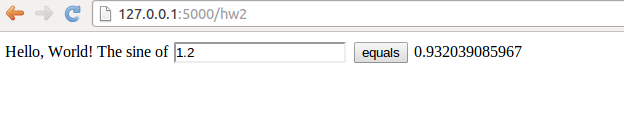
\includegraphics[width=0.9\linewidth]{fig-web4sa/hw2_flask_output.png}}
  \caption{
  The modified result page. \label{wf:hw2:flask:fig:result}
  }
\end{figure}
%\clearpage % flush figures wf:hw2:flask:fig:result


To let the user stay within the same page, we create a new directory \code{hw2_flask}
for this modified Flask app and copy the files from the previous
\code{hw1_flask} directory.  The idea now is to make use of just one
template, in \code{templates/view.html}:

\bhtmlpro
<form method=post action="">
  Hello, World! The sine of
  {{(form.r)}}
  <input type=submit value=equals>

{{s}}

</form>
\ehtmlpro

The form is identical to what we used in \code{view_input.html}, and the only
new thing is the value of \code{s}. We supply \code{s} as an object to the
\code{render_template} function and this object is available for
some programming in the HTML template. We can test on the value of \code{s}:
if it is \code{None}, we know that the computations are not performed and
\code{s} should not appear on the page, otherwise \code{s} holds the sine
value and we can write it out. The generated HTML code reads

\bhtml
<form method=post action="">
  Hello, World! The sine of
  <input id="r" name="r" type="text" value="1.2">
  <input type=submit value=equals>

0.932039085967

</form>
\ehtml

The \code{index} function needs adjustments since we use the same
template for the input and the output page:

\bpycod
# View
@app.route('/hw2', methods=['GET', 'POST'])
def index():
    form = InputForm(request.form)
    if request.method == 'POST' and form.validate():
        r = form.r.data
        s = compute(r)
    else:
        s = None

    return render_template("view.html", form=form, s=s)
\epycod
It is seen that if the user has given data, \code{s} is a \code{float}, otherwise
\code{s} is \code{None}. You are encouraged to test the app by running

\bsys
Terminal> python controller.py
\esys
and loading \code{http://127.0.0.1:5000/hw2} into your browser.
A nice little exercise is to control the formatting of the result \code{s}.
To this end, you transform \code{s} to a string: \code{s = '%.5f' % s} before
sending it to \code{render_template}.

\subsection{Splitting the app into model, view, and controller files}
\label{wf:hw3:flask}



\index{Flask!MVC pattern}

In our previous to Flask apps we have had the model, view, and
controller parts in one file \code{controller.py}. For illustration we
may split the previous \code{controller.py} into three files:
\code{model.py}, \code{view.py}, and \code{controller.py}, located in a
directory \code{hw3_flask}. The contents
in these files reflects the splitting introduced in the original
scienticic hello world program in Section~\ref{wf:hw:mvc}.
In the Flask context we have \code{model.py} as

\bpypro
from wtforms import Form, FloatField, validators

class InputForm(Form):
    r = FloatField(validators=[validators.InputRequired()])
\epypro

The view in 'view.py' consists of

\bpypro
from flask import Flask, render_template, request
from compute import compute

app = Flask(__name__)

@app.route('/hw3', methods=['GET', 'POST'])
def index():
    form = InputForm(request.form)
    if request.method == 'POST' and form.validate():
        r = form.r.data
        s = compute(r)
    else:
        s = None

    return render_template("view.html", form=form, s=s)
\epypro

The \code{controller.py} file finally runs the view's \code{app}:

\bpypro
from view import app

if __name__ == '__main__':
    app.run(debug=True)
\epypro

The statements are indentical to those in the \code{hw2_flask} app, only
the organization of the statement in files differ.


% !split
\subsection{Troubleshooting}

\index{Flask!troubleshooting}

\paragraph{Address already in use.}
You can easily kill the Flask application and restart it, but sometimes
you will get an error that the address is already in use.
To recover from this problem, run the \code{lsof} program to see which program
that applies the 5000 port (Flask runs its server on \code{http://127.0.0.1:5000}):

\bsys
Terminal> lsof -i :5000
COMMAND   PID USER   FD   TYPE  DEVICE SIZE/OFF NODE NAME
python  48824  hpl    3u  IPv4 1128848      0t0  TCP ...
Terminal> kill -9 48824
\esys
The last command killed the \code{python} job that ran the test server and
you are ready to relaunch the Flask application.

% !split
\section{Making a Django application}

Django applies two concepts, \emph{project} and \emph{application}. The application,
or app for short,
is the program we want to run through a web interface. The project is
a Python package containing common settings and configurations for
a collection of apps. This means that before we can make a Django app,
we must to establish a Django project.

\subsection{Installing Django}

\index{Django!installation}

We recommend to
download and istall the latest official version from
\href{{http://www.djangoproject.com/download/}}{\nolinkurl{http://www.djangoproject.com/download/}}. Pack out the tarfile, go
to the directory, and run \code{setup.py}:

\bsys
Terminal> tar xvzf Django-1.5-tar.gz
Terminal> cd Django-1.5
Terminal> sudo python setup.py install
\esys
The version in this example, 1.5, may be different at the time you
follow these instructions.


\subsection{Setting up a Django project}

\index{Django!making a project}

A Django project for managing a set of Django apps is
created by the command

\bsys
Terminal> django-admin.py startproject django_project
\esys
The result is a directory \code{django_project} whose content can be explored
by some \code{ls} and \code{cd} commands:

\bsys
Terminal> ls django_project
manage.py django_project
Terminal> cd django_project/django_project
Terminal> ls
__init__.py settings.py urls.py wsgi.py
\esys
The meaning of the generated files are briefly listed below.

\begin{enumerate}
  \item The outer \code{django_project/} directory is just a container for your project. Its name does not matter to Django.

  \item \code{manage.py} is a command-line utility that lets you interact with this Django project in various ways. You will typically run \code{manage.py} to launch a Django application.

  \item The inner \code{django_project/} directory is a Python package for the Django project. Its name is used in import statements in Python code (e.g., \code{import django_project.settings}).

  \item \code{django_project/__init__.py} is an empty file that just tells Python that this directory should be considered a Python package.

  \item \code{django_project/settings.py} contains the settings and configurations for this Django project.

  \item \code{django_project/urls.py} maps URLs to specific functions and thereby defines that actions that various URLs imply.

  \item \code{django_project/wsgi.py} is not needed in our examples.
\end{enumerate}

\noindent
Django comes with a web server for developing and debugging applications.
The server is started by running

\bsys
Terminal> python manage.py runserver
\esys
You will see that the server runs on the URL "http://127.0.0.1:8000/".
Load this URL into your browser to see a welcome message from Django,
meaning that the server is working.

Despite the fact that our web applications do not need a database, you
have to register a database with a Django project. To this end,
open the \code{django_project/settings.py} file in a text editor,
locate the \code{DATABASES} dictionary and make sure the following
code is there:

\bpycod
import os

def relative2absolute_path(relative_path):
    """Return the absolute path correspodning to relative_path."""
    dir_of_this_file = os.path.dirname(os.path.abspath(__file__))
    return os.path.join(dir_of_this_file, relative_path)

DATABASES = {
   'default' : {
      'ENGINE': 'django.db.backends.sqlite3',
      'NAME': relative2absolute_path('../database.db')
   }
}
\epycod
The \code{settings.py} file needs absolute paths to files, while it is
more convenient for us to specify relative paths. Therefore,
we made a function that figures out the absolute path to the \code{settings.py}
file and then combines this absolute path with the relative path.
The location and name of the database file can be chosen as desired.
Note that one should not use \code{os.path.join} to create paths as Django
applies the forward slash between directories also on Windows.


\subsection{Setting up a Django application}

\index{Django!making an application}

The next step is to create a Django app for our scientific hello
world program. We can place the app in any directory, but here we
utilize the following organization.
As neighbor to \code{django_project} we have
a directory \code{apps} containing our various scientific applications.
Under \code{apps} we create a directory \code{hw}
for the various versions of the scientific hello world applications:
\code{orig} for the original \code{hw.py} program, \code{mvc} for a split of this
program according to the original MVC pattern, \code{mvc_django} for
the MVC split according to the way Django requires,
and \code{hw1_django} for a first version of
the program with a Django-based web interface.

\bsys
Terminal> cd ..
Terminal> mkdir apps
Terminal> cd apps
Terminal> mkdir hw
Terminal> cd hw
Terminal> mkdir orig mvc
\esys
The file \code{hw.py} is moved to \code{orig} while \code{mvc} contains
the MVC refactored version with the files \code{model.py}, \code{view.py}, \code{compute.py},
and \code{controller.py}.

The \code{hw1_django} directory, containing the Django application, must be
made with
\bsys
Terminal> python ../../django_project/manage.py startapp hw1_django
\esys
The command creates a directory \code{hw1_django} with the content

\bsys
Terminal> cd hw1_django
Terminal> ls
__init__.py models.py tests.py views.py
\esys
The \code{__init__.py} file is empty and needed to ensure that the
Django application is a Python package. The other files are also
empty, but \code{models.py} and \code{views.py} will soon be filled with content.

At this point,
we need to register some information about our application in the
\code{django_project/settings.py} and \code{django_project/urls.py} files.

\paragraph{Step 1: Add the app.}
Locate the \code{INSTALLED_APPS}
tuple in \code{settings.py} and add your Django application as a Python package:
directory \code{django}:

\bpycod
INSTALLED_APPS = (
    'django.contrib.auth',
    'django.contrib.contenttypes',
    ...
    'hw1_django',
)
\epycod
However, Django will not be able to find the package \code{hw1_django}
unless we register the parent directory in \code{sys.path}:

\bpycod
import sys
sys.path.insert(0, relative2absolute_path('../../apps/hw'))
\epycod
Note here that the relative path is given with respect to the
location of the \code{settings.py} script.

\paragraph{Step 2: Adding a template directory.}
Make a subdirectory \code{templates} under \code{hw1_django},

\bsys
mkdir templates
\esys
and add the absolute path of this directory to the \code{TEMPLATE_DIRS} tuple:

\bpycod
TEMPLATE_DIRS = (
    relative2absolute_path('../../apps/hw/hw1_django/templates'),
)
\epycod
The \code{templates} directory will hold templates for the HTML code applied
in the web interfaces. The trailing comma is important (as this is
a tuple with only one element).

\paragraph{Step 3: Defining the URL.}
We need to connect the Django app with
an URL, i.e., the address we write into the web browser to launch the
app. Our app will be associated with a Python function \code{index}
in the \code{views} module within the \code{hw1_django} package.
Say we want the corresponding URL to
be named \code{hw}. This is registered in the \code{django_project/urls.py} file
by

\bpycod
urlpatterns = patterns('',
    url(r'^hw1/', 'hw1_django.views.index'),
\epycod
The first argument to the \code{url} function is a regular expression for
the URL and the second argument is the name of the function to call.
The name \code{index} resembles the \code{index.html} main page associated
with an URL, but any other name than \code{index} can be used.

% !split
\subsection{Programming the Django application}



The Django application is about filling the files \code{views.py} and \code{models.py}
with content. The mathematical computations are performed in \code{compute.py}
so we copy this file from the \code{mvc} directory to the \code{hw1_django} directory
for convenience (we could alternatively add \code{../mvc} to \code{sys.path} such that
\code{import compute} would work from the \code{hw1_django} directory).

\index{Django!input forms}
\index{Django!models.py@Django!{\rm\texttt{models.py}}}

\paragraph{The model.}
The \code{models.py} file contains the model which consists
of the data we need in the application, stored in Django's data types.
Our data consists of one number, called \code{r}, and \code{models.py} then
look like

\bpypro
from django.db import models
from django.forms import ModelForm

class Input(models.Model):
    r = models.FloatField()

class InputForm(ModelForm):
    class Meta:
        model = Input
\epypro
The \code{Input} class lists variables representing data as static class
attributes. The \code{django.db.models} module contains various classes
for different types of data, here we use \code{FloatField} to represent
a floating-point number (corresponding to a Python \code{float}).
The \code{InputForm} class has a the shown generic form across applications
if we by convention apply the name \code{Input} for the class holding the data.

\index{Django!index@Django!{\rm\texttt{index}} function}
\index{Django!views.py@Django!{\rm\texttt{views.py}}}

\paragraph{The view.}
The \code{views.py} file contains a function \code{index} which performs
the actions we want to perform when invoking
the URL ( here \code{http://127.0.0.1:8000/hw/}).
In addition, \code{views.py} has the \code{present_output} function from
the \code{view.py} file in the \code{mvc_django} directory.

\bpypro
from django.shortcuts import render_to_response
from django.template import RequestContext
from django.http import HttpResponse
from models import InputForm
from compute import compute

def index(request):
    if request.method == 'POST':
        form = InputForm(request.POST)
        if form.is_valid():
            form = form.save(commit=False)
            return present_output(form)
    else:
        form = InputForm()

    return render_to_response('hw1.html',
            {'form': form}, context_instance=RequestContext(request))

def present_output(form):
    r = form.r
    s = compute(r)
    return HttpResponse('Hello, World! sin(%s)=%s' % (r, s))
\epypro

The \code{index} function deserves some explanation. It must take one
argument, usually called \code{request}. There are two modes in the function. Either
the user has provided input on the web page, which means that
\code{request.method} equals \code{'POST'}, or we show a new web page
with which the user is supposed to interact.

\index{Django!HTML templates}

\paragraph{Making the input page.}
The input consists of a web form with
one field where we can fill in our \code{r} variable. This page
is realized by the two central statements

\bpycod
# Make info needed in the web form
form = InputForm()
# Make HTML code
render_to_response('hw1.html',
    {'form': form}, context_instance=RequestContext(request))
\epycod
The \code{hw1.html} file resides in the \code{templates} subdirectory and contains
a template for the HTML code:

\bhtmlpro
<form method="post" action="">
    Hello, World! The sine of {{ form.r }}
    <input type="submit" value="equals" />
</form>
\ehtmlpro
This is a \emph{template file} because it contains instructions like
\code{} and variables like \code{{{ form.r }}}. Django will
replace the former by some appropriate HTML statements, while the
latter simply extracts the numerical value of the variable \code{r} in
our form (specified in the \code{Input} class in \code{models.py}).
Typically, this \code{hw1.html} file
results in the HTML code

\bhtml
<form method="post" action="">
<div style='display:none'>
<input type='hidden' name='csrfmiddlewaretoken'
value='oPWMuuy1gLlXm9GvUZINv49eVUYnux5Q' /></div>
    Hello, World! The sine of <input type="text" name="r" id="id_r" />
    <input type="submit" value="equals" />
</form>
\ehtml
Figure~\ref{wf:hw1:django:fig:input} shows how the input page looks like in the
web browser.


\begin{figure}[ht]
  \centerline{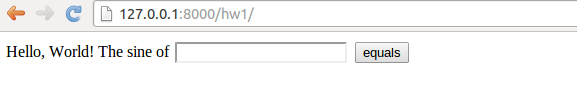
\includegraphics[width=0.9\linewidth]{fig-web4sa/hw1_django_input.png}}
  \caption{
  The input page. \label{wf:hw1:django:fig:input}
  }
\end{figure}
%\clearpage % flush figures wf:hw1:django:fig:input


\paragraph{Making the results page.}
When then user has filled in a value in the text field on the input
page, the \code{index} function is called again and \code{request.method} equals
\code{'POST'}. A new form object is made, this time with user info (\code{request.POST}).
We can check that the form is valid and if so, proceed with
computations followed by presenting the results in a
new web page (see Figure~\ref{wf:hw1:django:fig:result}):

\bpycod
def index(request):
    if request.method == 'POST':
        form = InputForm(request.POST)
        if form.is_valid():
            form = form.save(commit=False)
            return present_output(form)

def present_output(form):
    r = form.r
    s = compute(r)
    return HttpResponse('Hello, World! sin(%s)=%s' % (r, s))
\epycod
The numerical value of \code{r} as given by the user is available as \code{form.r}.
Instead of using a template for the output page, which is natural to
do in more advanced cases, we here illustrate the possibility to
send raw HTML to the output page by returning an \code{HttpResponse}
object initialized by a string containing the desired HTML code.


\begin{figure}[ht]
  \centerline{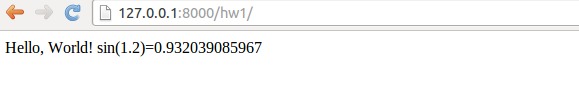
\includegraphics[width=0.9\linewidth]{fig-web4sa/hw1_django_output.png}}
  \caption{
  The result page. \label{wf:hw1:django:fig:result}
  }
\end{figure}
%\clearpage % flush figures wf:hw1:django:fig:result


Launch this application by filling in the address \code{http://127.0.0.1:8000/hw/}
in your web browser (make sure the Django development server is running,
and if not, restart it by \code{python manage.py runserver}). Try to fill
in some number on the input page and view the output.
To show how easy it is to change the application, invoke the \code{views.py}
file in an editor and add some color to the output HTML code from
the \code{present_output} function:

\bpycod
    return HttpResponse("""
<font color='blue'>Hello</font>, World!
sin(%s)=%s
"""% (r, s))
\epycod
Go back to the input page, provide a new number, and observe how
the "Hello" word now has a blue color.


\subsection{Equipping the input page with output results}



Instead of making a separate output page with the result, we can
simply add the sine value to the input page. This makes the user
feel that she interacts with the same page, as when operating a calculator.
The output page should then look as shown in Figure~\ref{wf:hw2:django:fig:result}.


\begin{figure}[ht]
  \centerline{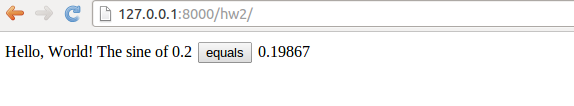
\includegraphics[width=0.9\linewidth]{fig-web4sa/hw2_django_output.png}}
  \caption{
  The modified result page. \label{wf:hw2:django:fig:result}
  }
\end{figure}
%\clearpage % flush figures wf:hw2:django:fig:result


We need to make a new Django application, now called \code{hw2_django}.
Instead of running
\code{manage.py startapp hw2_django} we can simply copy the \code{hw1_django}
directory. We need, of course, to add information about this
new application in \code{settings.py} and \code{urls.py}.
In the former file we must have

\bpycod
TEMPLATE_DIRS = (
    relative2absolute_path('../../apps/hw1_django/templates'),
    relative2absolute_path('../../apps/hw2_django/templates'),
)

INSTALLED_APPS = (
    'django.contrib.auth',
    'django.contrib.contenttypes',
    'django.contrib.sessions',
    'django.contrib.sites',
    'django.contrib.messages',
    'django.contrib.staticfiles',
    # Uncomment the next line to enable the admin:
    # 'django.contrib.admin',
    # Uncomment the next line to enable admin documentation:
    # 'django.contrib.admindocs',
    'hw1_django',
    'hw2_django',
)
\epycod
In \code{urls.py} we add the URL \code{hw2} which is to call our \code{index} function
in the \code{views.py} file of the \code{hw2_django} app:

\bpycod
urlpatterns = patterns('',
    url(r'^hw1/', 'hw1_django.views.index'),
    url(r'^hw2/', 'hw2_django.views.index'),
\epycod

The \code{views.py} file changes a bit since we shall generate almost the same
web page on input and output. This makes the \code{present_output} function
unnatural, and everything is done within the \code{index} function:

\bpycod
def index(request):
    s = None  # initial value of result
    if request.method == 'POST':
        form = InputForm(request.POST)
        if form.is_valid():
            form = form.save(commit=False)
            r = form.r
            s = compute(r)
    else:
        form = InputForm()

    return render_to_response('hw2.html',
            {'form': form,
             's': '%.5f' % s if isinstance(s, float) else ''
             }, context_instance=RequestContext(request))
\epycod

Note that the output variable \code{s} is computed within the \code{index}
function and defaults to \code{None}. The template file \code{hw2.html}
looks like

\bhtmlpro
<form method="post" action="">
    Hello, World! The sine of {{ form.r }}
    <input type="submit" value="equals" />

{{ s }}

</form>
\ehtmlpro
The difference from \code{hw1.html} is that we right after the \emph{equals}
button write out the value of \code{s}. However, we make a test that
the value is only written if it is computed, here recognized by
being a non-empty string. The \code{s} in the template file
is substituted by value corresponding to the key \code{'s'} in the
dictionary we pass to the \code{render_to_response}. As seen,
we pass a string where \code{s} is formatted with five digits if \code{s}
is a float, i.e., if \code{s} is computed. Otherwise, \code{s} has the
default value \code{None} and we send an empty string to the template.


% !split
\section{Handling multiple input variables in Flask}
\label{wf:vib:flask}

The scientific hello world example shows how to work with one input
variable and one output variable. We can easily derive a solution for
a collection of input variables and some corresponding HTML code
as result. Multiple input variables are listed in the \code{InputForm}
class using different types for different forms (text field,
float field, integer field, check box field for boolean values, etc.).
The value of these variables will be available in a \code{form} object
for computation. It is then a matter of taking the output from the
computation and format the corresponding HTML code for presenting
the result.

We address the task of plotting the function $u(t)=Ae^{-bt}\sin (wt)$ for
$t\in [0,T]$. The web application must have fields for the numbers $A$,
$b$, $w$, and $T$, and a \emph{Compute} button, as shown in Figure~\ref{wf:vib1:flask:fig:input}. Filling in values, say $0.1$ for $b$ and
$20$ for $T$, results in what we see in Figure~\ref{wf:vib1:flask:fig:result},
i.e., a plot of $u(t)$ is added after the input fields and the \emph{Compute}
button.


\begin{figure}[ht]
  \centerline{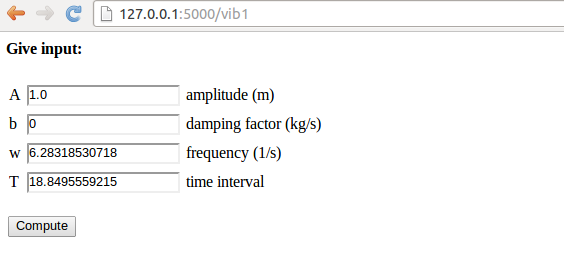
\includegraphics[width=0.9\linewidth]{fig-web4sa/vib1_flask_input.png}}
  \caption{
  The input page. \label{wf:vib1:flask:fig:input}
  }
\end{figure}
%\clearpage % flush figures wf:vib1:flask:fig:input



\begin{figure}[ht]
  \centerline{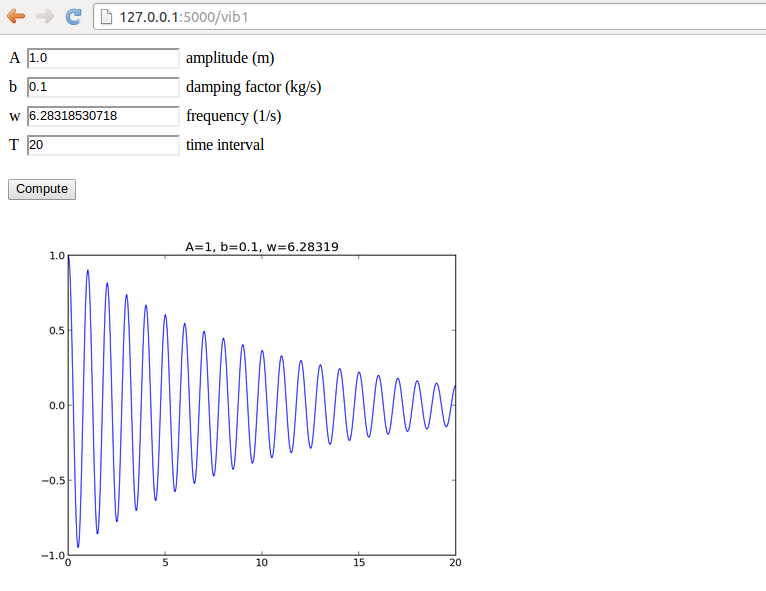
\includegraphics[width=0.9\linewidth]{fig-web4sa/vib1_flask_output.png}}
  \caption{
  The result page. \label{wf:vib1:flask:fig:result}
  }
\end{figure}
%\clearpage % flush figures wf:vib1:flask:fig:result


\subsection{Programming the Flask application}



The forthcoming text explains the necessary steps to realize a
Flask app that behaves as depicted in Figures~\ref{wf:vib1:flask:fig:input}
and~\ref{wf:vib1:flask:fig:result}. We start with the
\code{compute.py} module since it contains only the computation of $u(t)$
and the making of the plot, without any interaction with Flask.

More specifically, inside \code{compute.py}, we have a function for
evaluating $u(t)$ and a \code{compute} function for making the plot. The
return value is the name of the plot file, which should get a unique
name every time the \code{compute} function is called such that the browser
cannot reuse an already cached image. Flask applications must have all
extra files (CSS, images, etc.) in a subdirectory \code{static}.

\bpypro
from numpy import exp, cos, linspace
import matplotlib.pyplot as plt
import os, time, glob

def damped_vibrations(t, A, b, w):
    return A*exp(-b*t)*cos(w*t)

def compute(A, b, w, T, resolution=500):
    """Return filename of plot of the damped_vibration function."""
    t = linspace(0, T, resolution+1)
    y = damped_vibrations(t, A, b, w)
    plt.figure()  # needed to avoid adding curves in plot
    plt.plot(t, y)
    plt.title('A=%g, b=%g, w=%g' % (A, b, w))
    if not os.path.isdir('static'):
        os.mkdir('static')
    else:
        # Remove old plot files
        for filename in glob.glob(os.path.join('static', '*.png')):
            os.remove(filename)
    # Use time since Jan 1, 1970 in filename in order make
    # a unique filename that the browser has not chached
    plotfile = os.path.join('static', str(time.time()) + '.png')
    plt.savefig(plotfile)
    return plotfile

if __name__ == '__main__':
    print compute(1, 0.1, 1, 20)
\epypro

\index{Flask!input forms}

We organize the model, view, and controller as three separate
files, as illustrated in
Section~\ref{wf:hw3:flask}. This more complicated app involves
more code and especially the model will soon be handy to isolate in its own
file. Our first version of \code{model.py} reads

\bpypro
from wtforms import Form, FloatField, validators
from math import pi

class InputForm(Form):
    A = FloatField(
        label='amplitude (m)', default=1.0,
        validators=[validators.InputRequired()])
    b = FloatField(
        label='damping factor (kg/s)', default=0,
        validators=[validators.InputRequired()])
    w = FloatField(
        label='frequency (1/s)', default=2*pi,
        validators=[validators.InputRequired()])
    T = FloatField(
        label='time interval (s)', default=18,
        validators=[validators.InputRequired()])
\epypro

As seen, the field classes can take a \code{label} argument for a longer
description, here also including the units in which the variable is
measured. It is also possible to add a \code{description} argument with
some help message. Furthermore, we include a \code{default} value, which
will appear in the text field such that the user does not need to
fill in all values.

\index{Flask!index@Flask!{\rm\texttt{index}} function}

The view will of course make use of templates, and we shall experiment
with different templates. Therefore, we allow a command-line argument
to this Flask app for choosing which template we want. The rest of
the \code{view.py} file follows much the same set up as for the scientific
hello world app:

\bpypro
from model import InputForm
from flask import Flask, render_template, request
from compute import compute
import sys

try:
    template_name = sys.argv[1]
except IndexError:
    template_name = 'view0'

app = Flask(__name__)

@app.route('/vib1', methods=['GET', 'POST'])
def index():
    form = InputForm(request.form)
    if request.method == 'POST' and form.validate():
        result = compute(form.A.data, form.b.data,
                         form.w.data, form.T.data)
    else:
        result = None

    return render_template(template_name + '.html',
                           form=form, result=result)
\epypro

The details governing how the web page really looks like lie in the
template file. Since we have several fields and want them nicely
align in a tabular fashion, we place the field name, text areas,
and labels inside an HTML table in our first attempt to write a
template, \code{view0.html}:

\bhtmlpro
<form method=post action="">
<table>
  
    <tr>
    <td>{{ field.name }}</td><td>{{ field }}</td>
    <td>{{ field.label }}</td>
    </tr>
  
</table>
<p><input type=submit value=Compute></form></p>

<p>

<img src="{{ result }}" width=500>

</p>
\ehtmlpro
Observe how easy it is to iterate over the \code{form} object and grab data
for each field: \code{field.name} is the name of the variable in the
\code{InputForm} class, \code{field.label} is the full name with units as given
through the \code{label} keyword when constructing the field object, and
writing the field object itself generates the text area for
input (i.e., the HTML input form). The control statements we can
use in the template are part of the \href{{http://jinja.pocoo.org/docs/}}{Jinja2}
\emph{templating language}. For now, the if-test, for-loop and
output of values (\code{{{ object }}}) are enough to generate the HTML
code we want.

Recall that the objects we need in the template, like \code{result} and \code{form}
in the present case, are transferred to the template via keyword
arguments to the \code{render_template} function. We can easily pass on
any object in our application to the template.

To get a runnable Flask application it remains to
run the \code{app} object from \code{controller.py}:

\bpypro
from view import app

if __name__ == '__main__':
    app.run(debug=True)
\epypro

You are encouraged to run \code{python controller.py} and load \code{http://127.0.0.1:5000/vib1} into your web browser for testing.

% !split
\subsection{Implementing error checking in the template}

\index{Flask!error checking}

What happens if the user gives wrong input, for instance the letters \code{asd}
instead of a number? Actually nothing! The \code{FloatField} object
checks that the input is compatible with a real number in the
\code{form.validate()} call, but returns just \code{False} if this is not
the case. Looking at the code in \code{view.py},

\bpycod
def index():
    form = InputForm(request.form)
    if request.method == 'POST' and form.validate():
        result = compute(form.A.data, form.b.data,
                         form.w.data, form.T.data)
    else:
        result = None
\epycod
we realize that wrong input implies \code{result = None} and no computations
and plot. Fortunately, each field object gets an attribute \code{error}
with information on errors that occur on input. We can write out
this information on the web page, as exemplified in the template
\code{view1.html}:

\bhtmlpro
<form method=post action="">
<table>
  
    <tr>
    <td>{{ field.name }}</td><td>{{ field(size=12) }}</td>
    <td>{{ field.label }}</td>
    
      <td><ul class=errors>
      
        <li><font color="red">{{ error }}</font></li>
      </ul></td>
    
    </tr>
  
</table>
<p><input type=submit value=Compute></form></p>
<p>

<h4>Plot:</h4>
<img src="{{ result }}" width=500>

</p>
\ehtmlpro
Two things are worth noticing here:

\begin{enumerate}
\item We can control the width of the text field where the
   user writes the numbers, here set to 12 characters.

\item We can make an extra column in the HTML table with a list
   of possible errors for each field object.
\end{enumerate}

\noindent
Let us test the \code{A} field by writing \code{asd} instead of a number. This
triggers an error, which is written in red to the right of the label,
see Figure~\ref{wf:vib2:flask:fig:error1}.


\begin{figure}[ht]
  \centerline{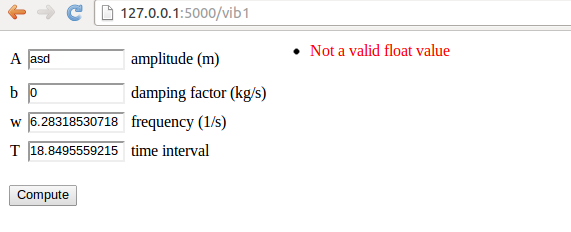
\includegraphics[width=0.9\linewidth]{fig-web4sa/vib1_flask_error1.png}}
  \caption{
  Error message because of wrong input. \label{wf:vib1:flask:fig:error1}
  }
\end{figure}
%\clearpage % flush figures wf:vib1:flask:fig:error1


% !split
\subsection{Using style sheets}

\index{Flask!CSS style sheets}

Web developers make heavy use of CSS style sheets to control the look
and feel of web pages. Templates can utilize style sheets as any other
standard HTML code. Here is a very simple example where we introduce
a class \code{name} for the column with the field name and set the
foreground color of the text in this column to blue.
The style sheet is called \code{basic.css} and \emph{must} reside in the
\code{static} subdirectory of the Flask application directory:

\bpro
td.name { color: blue; }
\epro
The \code{view2.html} file using this style sheet features a \code{link} tag
to the style sheet in the HTML header, and the column containing
the field name has
the HTML tag \code{<td class="name">} to trigger the specification in
the style sheet:

\bhtmlcod
<html>
<head>
<link rel="stylesheet" href="static/basic.css" type="text/css">
</head>
<body>

<form method=post action="">
<table>
  
    <tr>
    <td class="name">{{ field.name }}</td>
    <td>{{ field(size=12) }}</td>
    <td>{{ field.label }}</td>
\ehtmlcod
Just run \code{python controller.py view2} to see that the names
of the variables to set in the web page are blue.

\subsection{Using {\LaTeX} mathematics}

\index{Flask!{\LaTeX} mathematics}

Scientific applications frequently have many input data that are
defined through mathematics and where the typesetting on the
web page should be as close as possible to the typesetting where
the mathematics is explained. In the present example we would like
to typeset $A$, $b$, $w$, and $T$ with italic font as done
in {\LaTeX}. Fortunately, native {\LaTeX} typesetting is available in
HTML through the tool \href{{http://www.mathjax.org/}}{MathJax}.
Our template \code{view3.html} enables MathJax. Formulas are written
with standard {\LaTeX} inside \code{\(} and \code{\)}, while equations are surrounded
by \code{$$}. Here we use formulas exclusively:

\bhtmlcod
<script type="text/x-mathjax-config">
MathJax.Hub.Config({
  TeX: {
     equationNumbers: {  autoNumber: "AMS"  },
     extensions: ["AMSmath.js", "AMSsymbols.js", "autobold.js"]
  }
});
</script>
<script type="text/javascript"
 src="http://cdn.mathjax.org/mathjax/latest/MathJax.js?config=TeX-AMS-MML_HTMLorMML">
</script>

This web page visualizes the function \(
u(t) = Ae^{-bt}\sin (w t), \hbox{ for } t\in [0,T]
\).

<form method=post action="">
<table>
  
    <tr>
    <td>\( {{ field.name }} \)</td><td>{{ field(size=12) }}</td>
    <td>{{ field.label }}</td>
\ehtmlcod
Figure~\ref{wf:vib1:flask:fig:latex} displays how the
{\LaTeX} rendering looks like in the browser.


\begin{figure}[ht]
  \centerline{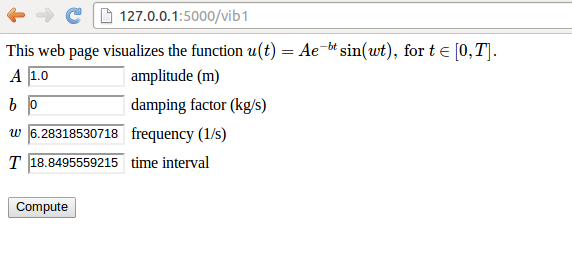
\includegraphics[width=0.9\linewidth]{fig-web4sa/vib1_flask_latex.png}}
  \caption{
  {\LaTeX} typesetting of mathematical symbols. \label{wf:vib1:flask:fig:latex}
  }
\end{figure}
%\clearpage % flush figures wf:vib1:flask:fig:latex



\subsection{Rearringing the elements in the HTML template}

Now we want to place the plot to the right of the input forms in
the web page, see Figure~\ref{wf:vib1:flask:fig:sidebyside}. This can
be accomplished by having an outer table with two rows. The first
row contains the table with the input forms in the first column and
the plot in the second column, while the second row features the
\emph{Compute} button in the first column.


\begin{figure}[ht]
  \centerline{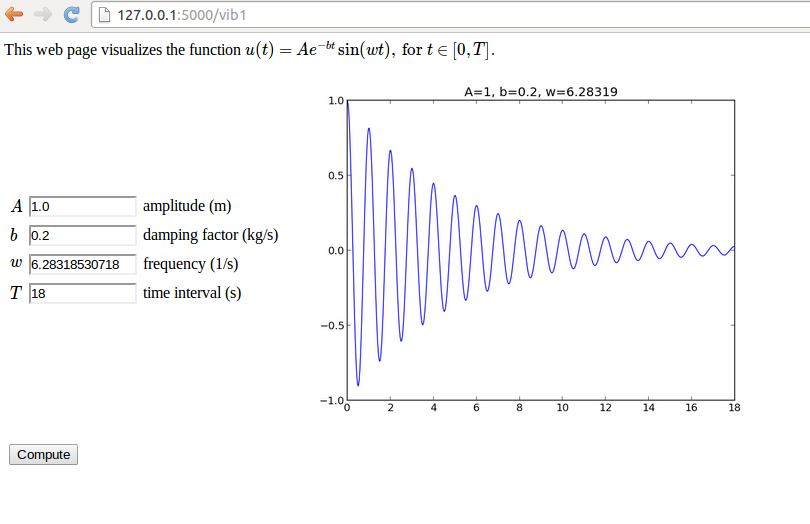
\includegraphics[width=0.9\linewidth]{fig-web4sa/vib1_flask_table2.png}}
  \caption{
  New design with input and output side by side. \label{wf:vib1:flask:fig:sidebyside}
  }
\end{figure}
%\clearpage % flush figures wf:vib1:flask:fig:sidebyside


A relevant template file is \code{view4.html}:

\bhtmlpro
<script type="text/x-mathjax-config">
MathJax.Hub.Config({
  TeX: {
     equationNumbers: {  autoNumber: "AMS"  },
     extensions: ["AMSmath.js", "AMSsymbols.js", "autobold.js"]
  }
});
</script>
<script type="text/javascript"
 src="http://cdn.mathjax.org/mathjax/latest/MathJax.js?config=TeX-AMS-MML_HTMLorMML">
</script>

This web page visualizes the function \(
u(t) = Ae^{-bt}\sin (w t), \hbox{ for } t\in [0,T]
\).

<form method=post action="">
<table> <!-- table with forms to the left and plot to the right -->
<tr><td>
<table>
  
    <tr>
    <td>\( {{ field.name }} \)</td><td>{{ field(size=12) }}</td>
    <td>{{ field.label }}</td>
    
      <td><ul class=errors>
      
        <li><font color="red">{{ error }}</font></li>
      </ul></td>
    
    </tr>
  
</table>
</td>
<td>
<p>

<img src="{{ result }}" width=500>

</p>
</td></tr>
<tr>
<td><p><input type=submit value=Compute></form></p></td>
</tr>
</table>
\ehtmlpro


% !split
\subsection{User-provided validation}



\index{Flask!input validation}


The \code{FloatField} objects can check that the input is compatible with
a number, but what if we want to control that $A>0$, $b>0$, and
$T$ is not greater than 30 periods (otherwise the plot gets cluttered)?
We can write functions for checking appropriate conditions and
supply the function to the list of validator functions in the call to
the \code{FloatField} constructor or other field constructors. The extra
code is a part of the \code{model.py} and the presented extensions appear
in the directory \code{vib2_flask}.

The simplest approach to validation is to use existing functionality
in the web framework. Checking that $A>0$ can be done by
the \code{NumberRange} validator which checks that the value is inside
a prescribed interval:

\bpycod
from wtforms import Form, FloatField, validators

class InputForm(Form):
    A = FloatField(
        label='amplitude (m)', default=1.0,
        validators=[validators.NumberRange(0, 1E+20)])
\epycod

We can also easily provide our own more tailored validators.
As an example, let us explain how we can check that $T$ is less than 30 periods.
One period is $2\pi /w$ so we need to check if $T> 30\cdot 2\pi/w$
and raise an exception in that case.
A validation function takes two arguments: the whole \code{form} and the
specific \code{field} to test:

\bpycod
def check_T(form, field):
    """Form validation: failure if T > 30 periods."""
    w = form.w.data
    T = field.data
    period = 2*pi/w
    if T > 30*period:
        num_periods = int(round(T/period))
        raise validators.ValidationError(
            'Cannot plot as much as %d periods! T<%.2f' %
            (num_periods, 30*period))
\epycod
The appropriate exception is of type \code{validators.ValidationError}.
Observe that through \code{form} we have in fact access to all the input
data so we can easily use the value of $w$ when checking the validity
of the value of $T$. The \code{check_T} function is easy to
add to the list of validator functions in the call to the \code{FloatField}
constructor for \code{T}:

\bpycod
class InputForm(Form):
    ...
    T = FloatField(
        label='time interval', default=6*pi,
        validators=[validators.InputRequired(), check_T])
\epycod
The validator
objects are tested one by one as the appear in the list, and if
one fails, the others are not invoked.
We therefore add \code{check_T} after the check of input such that we know we
have a value for all data when we run the computations and test
in \code{check_T}.

Although there is already a \code{NumberRange} validator for checking
whether a value is inside an interval, we can write our own
version with some improved functionality for open intervals where
the maximum or minimum value can be infinite.
The infinite value can on input be represented by \code{None}.
A general such function may take the form

\bpycod
def check_interval(form, field, min_value=None, max_value=None):
    """For validation: failure if value is outside an interval."""
    failure = False
    if min_value is not None:
        if field.data < min_value:
            failure = True
    if max_value is not None:
        if field.data > max_value:
            failure = True
    min_value = '-infty' if min_value is None else str(min_value)
    max_value =  'infty' if max_value is None else str(max_value)
    if failure:
        raise validators.ValidationError(
            '%s=%s not in [%s, %s]' % (field.name, field.data,
                                       min_value, max_value))
\epycod

\index{functools@{\rm\texttt{functools}}}

The problem is that \code{check_interval} takes four arguments, not only
the \code{form} and \code{field} arguments that a validator function can accept.
The way out of this difficulty is to use a Python tool \code{functools.partial}
which allows us to call a function with some of the arguments set.
Here, we want to create a new function that calls \code{check_interval}
with some prescribed values of \code{min_value} and \code{max_value}.
This function looks like it does not have these arguments, only
\code{form} and \code{field}. The following function produces this function:

\bpycod
import functools

def interval(min_value=None, max_value=None):
    return functools.partial(
        check_interval, min_value=min_value, max_value=max_value)
\epycod
We can in any field constructor just add
\code{interval(a, b)} as a validator function checking if the field value is
in the interval between \code{a} and \code{b}:

\bpycod
class InputForm(Form):
    ...
    b = FloatField(
        label='damping factor (kg/s)', default=0,
        validators=[validators.InputRequired(), interval(0,None)])
\epycod

Let us test our tailored error checking. Run \code{python controller.py}
in the \code{vib2_flask} directory and fill in $-1.0$ in the $b$ field.
Pressing \emph{Compute} invokes our \code{interval(0,None)} function, which
is nothing but a call \code{check_interval(field, form, 0, None)},
and the test \code{if field.data < min_value} becomes true, \code{failure}
is set and the exception is raised. The message in the exception
is available in the \code{field.errors} attribute so our template
will write it out in red, see Figure~\ref{wf:vib2:flask:fig:error1}.
The template used in \code{vib_flask} is basically the same as \code{view3.html}
in \code{vib1_flask}, i.e., it feaures {\LaTeX} mathematics and checking of
\code{field.errors}.


\begin{figure}[ht]
  \centerline{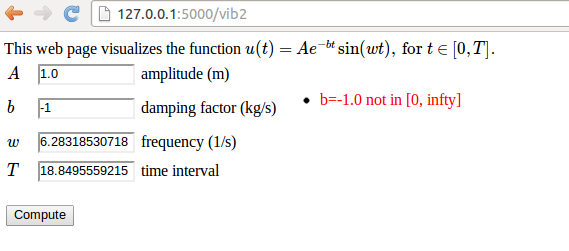
\includegraphics[width=0.9\linewidth]{fig-web4sa/vib2_flask_error1.png}}
  \caption{
  Triggering of a user-defined error check. \label{wf:vib2:flask:fig:error1}
  }
\end{figure}
%\clearpage % flush figures wf:vib2:flask:fig:error1


Finally, we mention a detail in the \code{view.py} file in the \code{vib2_flask}
app: instead of sending \code{form.var.data} to the \code{compute} function we
may automatically generate a set of local variables such that the
work with data from the web page looks nicer:

\bpycod
def index():
    form = InputForm(request.form)
    if request.method == 'POST' and form.validate():
        for field in form:
            # Make local variable (name field.name)
            exec('%s = %s' % (field.name, field.data))
        result = compute(A, b, w, T)
    else:
        result = None

    return render_template('view.html', form=form, result=result)
\epycod
The idea is just to run \code{exec} on a declaration of a local variable
with name \code{field.name} for each field in the form. This trick is often
neat if data are buried in objects and you want variables in your
code to look like they do in mathematical writing.

% !split
\subsection{Autogenerating the code}
\label{wf:vib3:flask:autogen}



\index{getattr@{\rm\texttt{getattr}}} \index{setattr@{\rm\texttt{setattr}}} \index{hasattr@{\rm\texttt{hasattr}}}

We shall now present generic \code{model.py}, \code{view.py}, and \code{controller.py}
files that work with \emph{any} \code{compute} function (!). This example will
demonstrate some advanced, powerful features of Python.

The basic idea is that the Python module \code{inspect} can be used to
retrieve the names of the arguments, and the default values of
keyword arguments of any given \code{compute} function. Say we have some

\bpycod
def mycompute(A, m=0, s=1, w=1, x_range=[-3,3]):
    ...
    return result
\epycod
Running

\bpycod
import inspect
arg_names = inspect.getargspec(mycompute).args
defaults  = inspect.getargspec(mycompute).defaults
\epycod
leads to

\bpycod
arg_names = ['A', 'm', 's', 'w', 'x_range']
defaults = (0, 1, 1, [-3, 3])
\epycod

Knowing the names \code{name} of some argument in the \code{compute}
function, we can make the corresponding class attribute
in the \code{InputForm} class by

\bpycod
setattr(InputForm, name, FloatForm())
\epycod
For name equal to \code{'A'} this is the same as hardcoding

\bpycod
class InputForm:
    A = FloatForm()
\epycod
Assuming that all arguments in \code{compute} are floats, we could
do

\bpycod
class InputForm:
    pass  # Empty class

arg_names = inspect.getargspec(mycompute).args
for name in arg_names:
    setattr(InputForm, name, FloatForm())
\epycod
However, we can do better than this: default values can be set for
keyword arguments, and the type of default value can be used to
select the appropriate form class. The complete \code{model.py} file
then goes as follows:

\bpypro
"""
Example on generic model.py file which inspects the arguments
of the compute function and automatically generates a relevant
InputForm class.
"""

import wtforms
from math import pi

from compute import compute_gamma as compute
import inspect
arg_names = inspect.getargspec(compute).args
defaults  = inspect.getargspec(compute).defaults

class InputForm(wtforms.Form):
    pass

# Augment defaults with None elements for the positional
# arguments
defaults = [None]*(len(arg_names)-len(defaults)) + list(defaults)
# Map type of default to right form field
type2form = {type(1.0): wtforms.FloatField,
             type(1):   wtforms.IntegerField,
             type(''):  wtforms.TextField,
             }

for name, value in zip(arg_names, defaults):
    if value is None:
        setattr(InputForm, name, wtforms.FloatField(
            validators=[wtforms.validators.InputRequired()]))
    else:
        if type(value) in type2form:
            setattr(InputForm, name, type2form[type(value)](
                default=value,
                validators=[wtforms.validators.InputRequired()]))
        else:
            raise TypeError('argument %s %s not supported' %
                            name, type(value))

if __name__ == '__main__':
    for item in dir(InputForm):
        if item in arg_names:
            print item, getattr(InputForm, item)
\epypro
(The \code{compute_gamma} function imported from \code{compute} will be treated later.)

The call to \code{compute} in the \code{view.py} file must also be expressed
in a general way such that it handle any type and number of
parameters. This is achieved by collecting all parameters in
a list or tuple, called \code{args}, and then calling \code{compute(*args)}
(which is equivalent to \code{compute(args[0], args[1], ..., args[l])}
if \code{l} is \code{len(args)-1}). The value of the form variable with
name \code{name} (string) is extracted by \code{getattr(form, name).data},
which is the same as \code{form.A.data} if \code{name} equals \code{'A'}.
Collecting all arguments and calling \code{compute} are done with

\bpycod
arg_names = inspect.getargspec(compute).args
args = [getattr(form, name).data for name in arg_names]
result = compute(*args)
\epycod
Our \code{InputForm} class guarantees that all arguments in \code{compute}
are present in the form, but to be absolutely safe we can
test if \code{name} is present in the \code{form} object:

\bpycod
args = [getattr(form, name).data for name in arg_names
        if hasattr(form, name)]
\epycod
We could also use keyword arguments in the call in case
the \code{args} list should have the parameters in the wrong order:

\bpycod
kwargs = {name: getattr(form, name).data for name in arg_names
          if hasattr(form, name)}
result = compute(**kwargs)
\epycod
The \code{compute(**kwargs)} becomes \code{compute(A=1, b=3, w=0.5)}
in case \code{kwargs = {'w'=0.5, 'A':1, 'b':3}} (recall that the order of
the keys in a Python dictionary is undetermined).

It remains to generate the right HTML template. The HTML code depends
what the returned \code{result} object from \code{compute} contains. Only the
writer of the \code{compute} function knows the details of the returned
result. Therefore, we leave it to this writer to provide the part
of the HTML template that renders the result. The file \code{templates/view_results.html} contains this user-provided code, while \code{templates/view_forms.html}
is the generic template for the forms:

\bhtmlpro
<form method=post action="">
<table>
  
    <tr><td>{{ field.name }}</td> <td>{{ field }}</td>
    <td>
      <ul class=errors>
      
        <li>{{ error }}</li>
      </ul>
    </td></tr>
  
</table>
<p><input type=submit value=Compute></form></p>
\ehtmlpro

By default, in \code{templates/view_results_default.html}, we can
create a code that checks if \code{results} is a string ending in \code{'.png'}
or other typical file extensions for HTML images, and then write out
the code for an image, and otherwise a string version of the \code{results}
object is dumped to the web page:

\bpypro
<p>

  
<img src="{{ result }}">
  
{{ str(result) }}
  

</p>
\epypro
The complete, generic \code{index} function now becomes

\bpycod
def index():
    form = InputForm(request.form)
    if request.method == 'POST' and form.validate():
        arg_names = inspect.getargspec(compute).args
        kwargs = {name: getattr(form, name).data
                  for name in arg_names if hasattr(form, name)}
        result = compute(**kwargs)
    else:
        result = None
    # Concatenate view_forms.html and view_results.html
    forms_html   = os.path.join('templates', 'view_forms.html')
    results_html = os.path.join('templates', 'view_results.html')
    view_html    = os.path.join('templates', 'view.html')
    f_forms = open(forms_html, 'r')
    f_res   = open(results_html, 'r')
    f_view  = open(view_html, 'w')
    f_view.write(f_forms.read() + f_res.read())
    f_forms.close();  f_res.close();  f_view.close()
    return render_template(os.path.basename(view_html),
                           form=form, result=result)
\epycod

\paragraph{Application.}
Let us apply the files above to plot the \emph{gamma probability density}

\[ g(x; a, h, A) = \frac{|h|}{\Gamma(a)A}\left(\frac{x}{A}\right)^{ah-1}
e^{-\left(\frac{x}{A}\right)^h},
\]
and its cumulative density

\[ G(x; a, h, A) = \int_0^x g(\tau; a, h, A)d\tau,\]
computed by numerically the Trapezoidal rule, for instance.
We also want to compute and display
the mean value $A\Gamma(a + 1/h)/\Gamma(a)$ and
standard deviation

\[ \sigma = \frac{A}{\Gamma(a)}\sqrt{\Gamma(a + 2/h)\Gamma(a) - Gamma(a+1/h)^2}.\]
Here, $\Gamma(a)$ is the gamma function, which can be computed
by \code{math.gamma(a)} using Python's \code{math} module.
Below are relevant implementations of $g(x;a,h,A)$ (\code{gamma_density}),
$G(x; a, h, A)$ (\code{gamma_cumulative}), and a function for
making a plot of $g$ og $G$ for $x\in [0,7\sigma]$.

\bpycod
def gamma_density(x, a, h, A):
    # http://en.wikipedia.org/wiki/Gamma_distribution
    xA = x/float(A)
    return abs(h)/(math.gamma(a)*A)*(xA)**(a*h-1)*exp(-xA**h)

def gamma_cumulative(x, a, h, A):
    # Integrate gamma_density using the Trapezoidal rule.
    # Assume x is array.
    g = gamma_density(x, a, h, A)
    r = zeros_like(x)
    for i in range(len(r)-1):
        r[i+1] = r[i] + 0.5*(g[i] + g[i+1])*(x[i+1] - x[i])
    return r

def compute_gamma(a=0.5, h=2, A=math.sqrt(2), resolution=500):
    """Return plot and mean/st.dev. value of the gamma density."""
    gah = math.gamma(a + 1./h)
    mean = A*gah/math.gamma(a)
    stdev = A/math.gamma(a)*math.sqrt(
        math.gamma(a + 2./h)*math.gamma(a) - gah**2)
    x = linspace(0, 7*stdev, resolution+1)
    y = gamma_density(x, a, h, A)
    plt.figure()  # needed to avoid adding curves in plot
    plt.plot(x, y)
    plt.title('a=%g, h=%g, A=%g' % (a, h, A))
    if not os.path.isdir('static'):
        os.mkdir('static')
    else:
        # Remove old plot files
        for filename in glob.glob(os.path.join('static', '*.png')):
            os.remove(filename)
    # Use time since Jan 1, 1970 in filename in order make
    # a unique filename that the browser has not chached
    t = str(time.time())
    plotfile1 = os.path.join('static', 'density_%s.png' % t)
    plotfile2 = os.path.join('static', 'cumulative_%s.png' % t)
    plt.savefig(plotfile1)
    y = gamma_cumulative(x, a, h, A)
    plt.figure()
    plt.plot(x, y)
    plt.grid(True)
    plt.savefig(plotfile2)
    return plotfile1, plotfile2, mean, stdev
\epycod
The \code{compute_gamma} function returns a tuple of four values.
We want output as displayed in Figure~\ref{wf:vib3:flask:fig:gamma}.


\begin{figure}[ht]
  \centerline{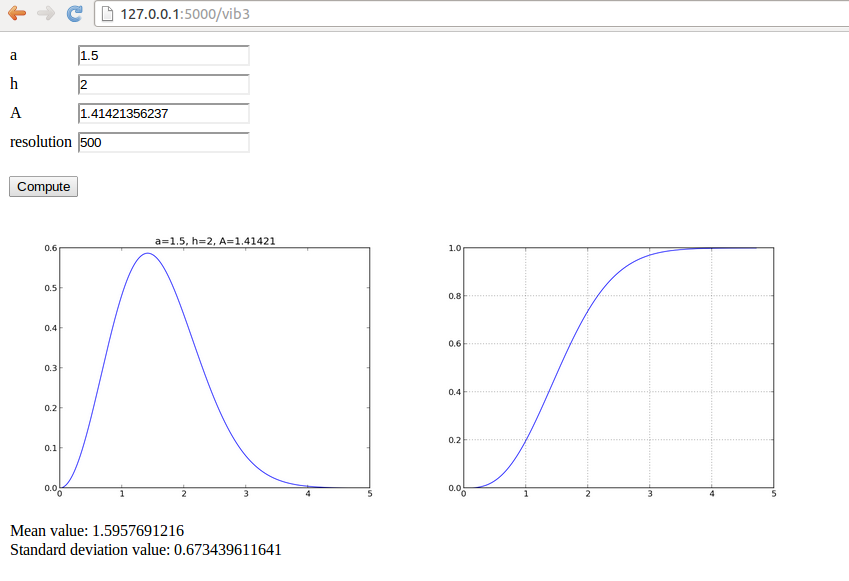
\includegraphics[width=0.9\linewidth]{fig-web4sa/vib3_flask_gamma.png}}
  \caption{
  Design of a web page illustrating the gamma probability functions. \label{wf:vib3:flask:fig:gamma}
  }
\end{figure}
%\clearpage % flush figures wf:vib3:flask:fig:gamma


The design is realized in the file \code{view_results.html} shown below.

\bhtmlpro

<p>
<table>
<tr>
<td><img src="{{ result[0] }}" width="400"></td>
<td><img src="{{ result[1] }}" width="400"></td>
</tr>
<tr><td>
Mean value: {{ result[2] }} <br>
Standard deviation value: {{ result[3] }}
</td></tr>
</table>
</p>

\ehtmlpro



% !split
\section{Handling multiple input variables in Django}
\label{wf:vib:django}

We shall briefly demonstrate how to make the multi-variable input
application from Section~\ref{wf:vib:flask} in Django.
There are four float input variables: $A$, $b$, $w$, and $T$.
A function \code{compute} in the file \code{compute.py} makes
a plot of a function depending on these four parameters and returns
the name of the plot file. Our task is to define four input fields,
execute the \code{compute} function and show the input fields together with
the resulting plot, cf.~Figures~\ref{wf:vib1:flask:fig:input}
and~\ref{wf:vib1:flask:fig:result}.

\subsection{Programming the Django application}




Any Django app needs a project, but here we reuse the project
we set up for the scientific hello world examples. We go to
\code{apps/vib} and create the Django app

\bsys
Terminal> python ../../django_project/manage.py startapp vib1_django
\esys
Then we

\begin{enumerate}
\item add \code{sys.path.insert(0, relative2absolute_path('../../apps/vib'))}
   in \code{settings.py},

\item add \code{relative2absolute_path('../../apps/vib/vib1_django/templates'),}
   to the \code{TEMPLATE_DIRS} tuple in \code{settings.py}, and

\item add \code{url(r'^vib1/', 'vib1_django.views.index')} to the \code{patterns}
   call in \code{urls.py}.
\end{enumerate}

\noindent
\index{Django!input forms}

We can now invoke \code{models.py} to add form fields for the four
input variables:

\bpypro
from django.db import models
from django.forms import ModelForm
from math import pi

class Input(models.Model):
    A = models.FloatField(
        verbose_name=' amplitude (m)', default=1.0)
    b = models.FloatField(
        verbose_name=' damping coefficient (kg/s)', default=0.0)
    w = models.FloatField(
        verbose_name=' frequency (1/s)', default=2*pi)
    T = models.FloatField(
        verbose_name=' time interval (s)', default=18)

class InputForm(ModelForm):
    class Meta:
        model = Input
\epypro
Note here that we can provide a more explanatory name than just
the variable name, e.g., \code{' amplitude (m)'} for \code{A}. However,
Django will always capitalize these descriptions, so if one really
needs lower case names (e.g., to be compatible with mathematics),
one must start the text with a space. We also provide a default
value such that all fields have a value when the user sees
the page.

\index{Django!index@Django!{\rm\texttt{index}} function}

The \code{views.py} file looks as follows:

\bpypro
from django.shortcuts import render_to_response
from django.template import RequestContext
from django.http import HttpResponse
from models import InputForm
from compute import compute
import os

def index(request):
    os.chdir(os.path.dirname(__file__))
    result = None
    if request.method == 'POST':
        form = InputForm(request.POST)
        if form.is_valid():
            form2 = form.save(commit=False)
            result = compute(form2.A, form2.b, form2.w, form2.T)
            result = result.replace('static/', '')
    else:
        form = InputForm()

    return render_to_response('vib1.html',
            {'form': form,
             'result': result,
             }, context_instance=RequestContext(request))
\epypro
Some remarks are necessary:

\begin{enumerate}
\item Doing an \code{os.chdir} to the current working directory is necessary
   as Django may be back in another working directory if you have
   tested other apps.

\item The \code{form2} object from \code{form.save} is the object we extract
   data from and send to \code{compute}, but the original \code{form}
   object is needed when making the HTML page through the template.

\item Images, media files, style sheets, javascript files, etc. must
   reside in a subdirectory \code{static}. The specifications of the
   URL applies tools to find this \code{static} directory and then
   the \code{static} prefix in the \code{result} filename must be removed.
\end{enumerate}

\noindent
The template for rendering the page is listed next.

\bhtmlpro
<form method=post action="">
<table>
  
    <tr>
    <td>{{ field.name }}</td>
    <td>{{ field }}</td>
    <td>{{ field.label }}</td>
    <td>{{ field.errors }}</td>
    <td></td>
    </tr>
  
</table>
<p><input type=submit value=Compute></form></p>

<p>


<img src="{{ result }}" width=500>

</p>
\ehtmlpro
The tricky part is the syntax for displaying \emph{static content}, such as
the plot file made in the \code{compute} function.

\subsection{User-provided validation}



Django has a series of methods available for user-provided validation
of form data. These are exemplified in the app \code{vib2_django}, which
is an extension of the \code{vib1_django} app (with additional code, and
of course, registrations in \code{settings.py} and \code{urls.py}).

\index{Django!input validation}

Checking that $A>0$ is easiest done with a built-in Django
validator:

\bpycod
class Input(models.Model):
    A = models.FloatField(
        verbose_name=' amplitude (m)', default=1.0,
        validators=[MinValueValidator(0)])
\epycod

We can write our own validators, which are functions taking one parameter
as argument, a value, and raising a \code{ValidationError} if the value
is wrong. Checking that a value is inside an interval can first be
implemented by

\bpycod
def check_interval(value, min_value=None, max_value=None):
    """Validate that a value is inside an interval."""
    failure = False
    if min_value is not None:
        if value < min_value:
            failure = True
    if max_value is not None:
        if value > max_value:
            failure = True
    min_value = '-infty' if min_value is None else str(min_value)
    max_value =  'infty' if max_value is None else str(max_value)
    if failure:
        raise ValidationError(
            'value=%s not in [%s, %s]' %
            (value, min_value, max_value))
\epycod
However, this function takes more than the value as argument. We therefore
need to wrap it by a function with \code{value} as the only argument:

\bpycod
import functools

def interval(min_value=None, max_value=None):
    """Django-compatible interface to check_interval."""
    return functools.partial(
        check_interval, min_value=min_value, max_value=max_value)
\epycod
Now, \code{interval(0, 1)} returns a function that takes \code{value} as its
only argument and checks if it is inside $[0,1]$.
Such a function can be inserted in the \code{validators} list in
the field constructor, here to tell that $b$ must be in $[0,\infty)$:

\bpycod
class Input(models.Model):
    ...
    b = models.FloatField(
        verbose_name=' damping coefficient (kg/s)', default=0.0,
        validators=[interval(0,None)])
\epycod

A final example on custom validation is to avoid plotting more
than 30 periods of the oscillating function $u$. This translates
to checking of $T$ is geater
than 30 periods, i.e., $T>30\cdot 2\pi/w$. The task is done in
the \code{InputForm} class, where any method \code{clean_T} can do
validation and adjustment of the field name \code{T}. The code goes
as follows:

\bpycod
class InputForm(ModelForm):
    class Meta:
        model = Input

    def clean_T(self):
        T = self.cleaned_data['T']
        w = self.cleaned_data['w']
        period = 2*pi/w
        if T > 30*period:
            num_periods = int(round(T/period))
            raise ValidationError(
                'Cannot plot as much as %d periods! T < %.2f' %
                (num_periods, 30*period))
        return T
\epycod
We refer to the vast Django documentation for many other ways of
validating forms.

% !split
\section{Exercises}



% --- begin exercise ---
\begin{exercise}
\refstepcounter{exerno}

\subsection*{Exercise 1: Add two numbers}
\label{wf:exer:add2}

Make a web application that reads two numbers from a web page,
adds the numbers, and prints the sum in a new web page.
Package the necessary files that constitute the application
in a tar file.
Filename: \code{add2.tar.gz}.

\end{exercise}
% --- end exercise ---


\section{Remaining}

\begin{itemize}
 \item apply (generated apps) to simviz (make py simviz too and describe that)

 \item store data in database

 \item discuss list values read as text and use of eval, perhaps exercise

 \item avoid Flask or Django in exercises, just do not specify and have
   common exercises at the very end

 \item app: username, TextAreaField, store in database and retrieve for admin
\end{itemize}

\noindent

% ------------------- end of main content ---------------


% #ifdef PREAMBLE
\printindex

\end{document}
% #endif

